\documentclass[pdftex, 11pt]{article}

\usepackage[pdftex]{graphicx}
\usepackage{listings}
\usepackage{fancyhdr}
\usepackage{lastpage}
\usepackage{fullpage}
\usepackage{color}
\usepackage[pdftex,bookmarks=true,colorlinks=true,linkcolor=blue]{hyperref}

%this sets the line at the header
\setlength{\headheight}{15.2pt}

\newcommand{\HRule}{\rule{\linewidth}{0.5mm}}

% This is all for formatting and making the Table of Contents according to 
% spec. Don't play with it.
\makeatletter
\renewcommand\l@section[2]{%
  \ifnum \c@tocdepth >\z@
    \addpenalty\@secpenalty
    \addvspace{1.0em \@plus\p@}%
    \setlength\@tempdima{1.5em}%
    \begingroup
      \parindent \z@ \rightskip \@pnumwidth
      \parfillskip -\@pnumwidth
      \leavevmode \bfseries
      \advance\leftskip\@tempdima
      \hskip -\leftskip
      #1\nobreak\ 
      \leaders\hbox{$\m@th\mkern \@dotsep mu\hbox{.}\mkern \@dotsep mu$}
     \hfil \nobreak\hb@xt@\@pnumwidth{\hss #2}\par
    \endgroup
  \fi}
\makeatother



\begin{document}
%import the title page
\begin{titlepage}
	\begin{center}

		% Upper part of the page
		\textsc{\LARGE University of Nevada, Reno}\\[.5cm]
		
\includegraphics[width=0.15\textwidth]{./logo.png}\\[.5cm]

		\textsc{\large CS 302 | Data Structures } \\[.5cm]

		% Title
		\HRule \\[0.4cm]
		{ \huge \bfseries Assignment \#3}\\[0.4cm]

		\HRule \\[1.5cm]

		% Author and supervisor
		\begin{minipage}{0.4\textwidth}
			\begin{flushleft} \large
				\emph{Students:}\\
				Joshua \textsc{Gleason}\\
				Josiah \textsc{Humphrey}
			\end{flushleft}
		\end{minipage}
		\begin{minipage}{0.4\textwidth}
			\begin{flushright} \large
				\emph{Instructor:} \\
				Dr. George \textsc{Bebis}
			\end{flushright}
		\end{minipage}

		\vfill

		% Bottom of the page
		{\large \today}

	\end{center}

\end{titlepage}


%headers, footers, and table of contents
\pagestyle{fancy}
\renewcommand{\sectionmark}[1]{\markright{\thesection}}
\rhead{Page \thepage\ of \pageref{LastPage}}
\lhead{}
\lfoot{CS 302 | Spring 2010}
\cfoot{}
\renewcommand{\footrulewidth}{0.4pt}

\tableofcontents
\newpage

\lhead{Joshua Gleason \& Josiah Humphrey}
\rhead{Page \thepage\ of \pageref{LastPage}}
\rfoot{Section\ \rightmark}
%\rfoot{Section\ \if\relax\thesubsection\relax \rightmark \else \thesection\fi}
\cfoot{}
\lfoot{CS 302 | Spring 2010}
\renewcommand{\footrulewidth}{0.4pt}

\section{Introduction}


\section{Use of Code}


\section{Functions}

\subsection{Image.h}
\begin{description}

	\item{\textsc{constructor}}
		\begin{description}
			\item{Purpose}

				default constructor allocates no memory and sets the size to zero 

			\item{Input}

				None

			\item{Output}

				None

			\item{Assumptions}

				Sets everything to zero and 
				sets the pixelValue array to NULL


		\end{description}


	\item{\textsc{constructor with parameters}}
		\begin{description}
			\item{Purpose}

				change the dimenstions of the image, delete,
				and re-allocate memory if required

			\item{Input}

				An N, M, and Q value to set the new image to

			\item{Output}

				None

			\item{Assumptions}

				Sets the image to a certain size and intializes the
				image as a grid

		\end{description}



	\item{\textsc{desctructor}}
		\begin{description}
			\item{Purpose}

				Deletes and memory that has been dynamically allocated

			\item{Input}

				None

			\item{Output}

				None

			\item{Assumptions}

				Checks to see if the pixelValue array has been set
				if so, deletes

		\end{description}


	\item{\textsc{copy\_constructor}}
		\begin{description}
			\item{Purpose}
		
				Creates a new array absed on the thing to be copied
				then sets the pixelValue of the new object the same as
				the old image

			\item{Input}

				ImageType rhs is the old image to be copied over into
				the new array


			\item{Output}

				None

			\item{Assumptions}

				The old image must be passed as reference to prevent
				an infinate loop


		\end{description}


	\item{\textsc{operator=}}
		\begin{description}
			\item{Purpose}

				equal operator overload, this is basically
				the same as the copy constructor
				except it will likely have to 
				de-allocate memory before copying values, all
				this is decided in setImageInfo however

			\item{Input}

				imageType rhs which is the old iamge to be 
				copied over to the new image

			\item{Output}

				Returns the imageType obejct so that
				equal chaining can be implemented


			\item{Assumptions}

				Assumes that the user is not trying to copy the same
				object into itself


		\end{description}


	\item{\textsc{getimageInfo}}
		\begin{description}
			\item{Purpose}
			
 				returns the width height and color depth 
				to reference variables

			\item{Input}

				\begin{itemize}
					\item{rows}

						This parameter grabs the number of rows
						in the imageType object

					\item{cols}

						This parameter grabs the number of cols
						in the imageType object

					\item{levels}

						This paremeter grabs the depth of the
						image in the imageType object

				\end{itemize}

			\item{Output}

				None

			\item{Assumptions}

				Assumes nothing but it makes sense that the object being
				queried has been loaded with some image



		\end{description}


	\item{\textsc{setImageInfo}}
		\begin{description}
			\item{Purpose}
			
				Sets the image info, deleting and allocating memory
				as required, also creates a background grid

			\item{Input}

				\begin{itemize}
					\item{rows}

						This parameter sets the number of rows
						in the imageType object

					\item{cols}

						This parameter sets the number of cols
						in the imageType object

					\item{levels}

						This paremeter sets the depth of the
						image in the imageType object

				\end{itemize}

			\item{Output}

				None

			\item{Assumptions}

				Assumes nothing

			\item{Example}

		\end{description}




	\item{\textsc{getpixelval}}
		\begin{description}
			\item{Purpose}

				Returns the value of a pixel

			\item{Input}

				\begin{itemize}

					\item{i}
					
						The row of the pixel

					\item{j} 

						The column of the pixel

				\end{itemize}

			\item{Output}

				The integer value of the pixel at 
				pixelValue[i][j]


			\item{Assumptions}

				It is assumed that the image has been intialized

			\item{Example}


		\end{description}


	\item{\textsc{setpixelval}}
		\begin{description}
			\item{Purpose}

				Sets the value of a pixel

			\item{Input}

				\begin{itemize}

					\item{i}

						The row of the pixel to be changed

					\item{j}

						The column of the pixel to be changed

				\end{itemize}

			\item{Output}

				None

			\item{Assumptions}

				Assumes the image has been intialized

			\item{Example}

		\end{description}


	\item{\textsc{getsubimage}}
		\begin{description}
			\item{Purpose}

 				Obtain a sub-image from old.  Uses the coordinates
				of the upper left corner
				and lower right corner to obtain image.

			\item{Input}

				\begin{itemize}

					\item{ULr}
	
						The upper left row of the pixel
						to be x in (0,0) in the new image.

					\item{ULc}

						The upper left column of the pixel
						to be y in (0,0) in the new image

					\item{LRr}

						The lower right row of the pixel
						to be x in (max\_x, max\_y) in the
						new image

					\item{LRC}

						The lower right row of the pixel
						to be y in (max\_x, max\_y) in the
						new image

				\end{itemize}


			\item{Output}

				None


			\item{Assumptions}

				Assumes that the UL\{r,c\} and LR\{r,c\} have been
				properly bounds and error checked before the function
				call

			\item{Example}

				
\includegraphics{images/outsubimg.png}

		\end{description}


	\item{\textsc{meangray}}
		\begin{description}
			\item{Purpose}

				
				this calculates the average gray value in the
				picture, this is done by adding
				all of the pixels and dividing by the total
				number of pixels

			\item{Input}

				None

			\item{Output}

				A double value that is the mean value of all
				the pixels in pixelValue


			\item{Assumptions}

				Assumes nothing and returns 0 if the image 
				has not been intialized

			\item{Example}


		\end{description}


	\item{\textsc{enlargeImage}}
		\begin{description}
			\item{Purpose}
				
				This function enlarges an image by a 
				magnitude of s, so for example if the
				original function was 100x100 and s is 
				10, then the new image is 1000x1000

			\item{Input}

				\begin{itemize}

					\item{S}

						This is the magnitude of the enlargement

						The function is also overloaded 
						to accept ints as well as doubles

					\item{ImageType old}

						This is the image to be enlarged

					\item{cubic}

						A bool value that decides which type of
						interpolation to use.
						If true, use cubic interpolation
						If false, use linear interpolation
				\end{itemize}

			\item{Output}

				None

			\item{Assumptions}


				The method choosen to use was bicubic/linear
				interpolation which creates
				splines for each column(cubic or linear),
				then using those splines create an
				image which is a stretched version of the original 
				image.  The way this was achieved
				was to stretch the entire image only vertically,
				and then stretch that
				image horizontally.  Then the same thing was done except
				reversed (stretched image
				horizontally first) and then the two image summed 
				together.  This gives an
				average value between both methods.  Although it can
				handle S values less
				than 1, the shrinkImage function works better for this.

		\end{description}

	\item{\textsc{shrinkImage}}
		\begin{description}
			\item{Purpose}

				Shrink image, average all the values
				in the block to make the new pixel, this
				makes the shrink much less jagged looking in the end

			\item{Input}

				\begin{itemize}

					\item{s}

						The inteter value of the shrink factor

					\item{ImageType old}

						The image to be shrunk

				\end{itemize}

			\item{Output}

				None

			\item{Assumptions}

				Assumes the image has been intialized and that error
				checking has been done.

			\item{Example}

				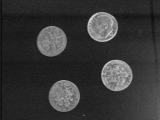
\includegraphics{images/outshrink.png}

		\end{description}


	\item{\textsc{reflectImage}}
		\begin{description}
			\item{Purpose}

				reflects image by moving the pixel to N or M
				minus the current row or column
				depending on the value of the flag
				(true being a horizontal reflection and
				false being a vertical reflection)

			\item{Input}

				\begin{itemize}

					\item{flag}

						The flag that sets either vertical or
						horizontal reflection

					\item{ImageType old}

						The image to be reflected

				\end{itemize}

			\item{Output}

				None

			\item{Assumptions}

				Assumes nothing, but it makes sense to have an intialized
				image to reflect

			\item{Example}

				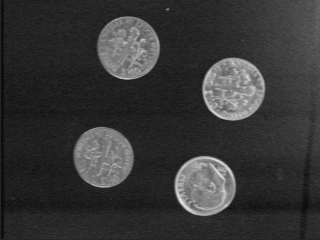
\includegraphics{images/outreflect.png}

		\end{description}


	\item{\textsc{translateImage}}
		\begin{description}
			\item{Purpose}

				Translate the image down to the right,
				any part that goes out of the screen is
 				not calculated.  Checkered background from
				setImageInfo is retained.

			\item{Input}

				\begin{itemize}

					\item{t}

						The integer value of the translation. The
						translation will occur down and 
						to the right 't' pixels

					\item{ImageType old}

						The image to be translated

				\end{itemize}

			\item{Output}

				None

			\item{Assumptions}

				No assumptions are made, but it makes sense to have
				an intialized image

			\item{Example}

				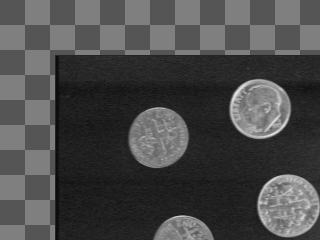
\includegraphics{images/outtrans.png}

		\end{description}


	\item{\textsc{rotateImage}}
		\begin{description}
			\item{Purpose}

				Rotate the image clockwise using bilinear
				interpolation, basically traversing
				the entire image going from the destination 
				to the source by using the
				in reverse (which is why its clockwise). 
				Once a location is determined the
				surrounding pixels are used to calculate 
				intermediate values between the
				pixels, this gives a pretty smooth rotate.

			\item{Input}

				\begin{itemize}

					\item{theta}

						The degrees to rotate. This is converted
						to radians inside the function

					\item{ImnageType old}

						The image to be rotated

				\end{itemize}

			\item{Output}

				None

			\item{Assumptions}

				Assumes that theta is in degrees because theta is
				converted to radians from degrees inside the function
				for the use of the trig functions.
				It is also assumed that the image has been intialized
				before the function call. It is also assumed that theta
				is between 0 and 360.

			\item{Example}

				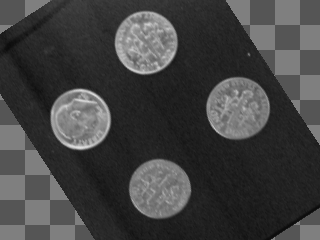
\includegraphics{images/outrotate.png}

		\end{description}


	\item{\textsc{operator+}}
		\begin{description}
			\item{Purpose}

				
				Sum two images together, basically just finding
				the average pixel value of
				every pixel between two images.  Throws an
				exception if dimesions of both
				images don't match

			\item{Input}

				\begin{itemize}
						
					\item{ImageType rhs}

						This is the image to be added to
						'this' image

				\end{itemize}

			\item{Output}

				ImageType object to chain additions

			\item{Assumptions}

				It is assumed that each image have the same dimensions.
				However, if the images do not have the same dimensions,
				then a string is thrown stating that the images do
				not have the same dimensions. It is not neccesary to have
				each image initialized, but it makes senses
				that they would each be initialized.

			\item{Example}

				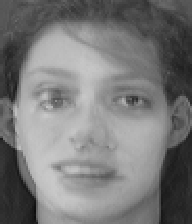
\includegraphics{images/outasum.png}

		\end{description}


	\item{\textsc{operator-}}
		\begin{description}
			\item{Purpose}

				subtract two images from each other to see the 
				differences, if the magnitude of
				the difference is less then Q/6 then the pixel
				is replaced with black,	otherwise white is used. 
				This seems to help reduce 
				the amount of noise in the pictures

			\item{Input}

				\begin{itemize}

					\item{ImageType rhs}

						This is the image to be subtracted from
						'this' image

				\end{itemize}

			\item{Output}

				ImageType is returned to allow chaining of subtraction

			\item{Assumptions}

				It is assumed that each image have the same dimensions.
				However, if the images do not have the same dimensions,
				then a string is thrown stating that the images do
				not have the same dimensions. It is not neccesary to have
				each image initialized, but it makes senses
				that they would each be initialized.

			\item{Example}

				
\includegraphics{images/outsubtract.png}

		\end{description}


	\item{\textsc{negateImage}}

\end{description}

\subsection{driver.cpp}

\begin{description}

	\item{\textsc{showmenu}}

		\begin{description}
			\item{Purpose}
				
 				This is the function which builds the scrolling menu system, this simply
				creates a curses window and puts all the options stored in menuStr onto the
				window, it then waits for the user to press UP, DOWN, or RETURN before
				reacting.  The parameters allow menus to be different widths, heights, and
				locations.  A few constants can be changed to change the colors of the window.

			\item{Input}

				An un-initialized window pointer, a string to be the title,
				height, width, xLoc, yLoc of the window, list of c-style
			   	strings to be used in the menu, the number of menu options,
				and a bool value which says weather the last choice is
				left highlighted.

			\item{Output}
				
				Display a window with menu options, let user choose and
				return the index of that choice.

			\item{Assumptions}

				Assumes that window is un-intialized and will be destructed
				by calling function.

		\end{description}


	\item{\textsc{showregs}}

		\begin{description}
			\item{Purpose}

 				Display a window of registers next to the main menu (or wherever the constants
				dictate).

			\item{Input}

				An un-initialized window pointer, a title string, and a
				list of register names.

			\item{Output}

				Displays a window next to main of all the registers.

			\item{Assumptions}

				This allocates memeory for a WINDOW but it doesn't delete it.

		\end{description}


	\item{\textsc{drawwindow}}

		\begin{description}
			\item{Purpose}

				This function simply draws an empty window with a given title, height, width,
				x, and y locations.  The colors have default values but can be changed if
				oddly colored windows are wanted.

			\item{Input}

				An un-intialized window pointer, a title string, and then
				the window height, width, yLoc, and xLoc, plus the colors
				for the background and foreground which are defaulted to some constants.

			\item{Output}

				Displays a empty window with a border and title using the
				given parameters.

			\item{Assumptions}

				This allocates memeory for a WINDOW but it doesn't delete it.

		\end{description}


	\item{\textsc{deletemenu}}

		\begin{description}
			\item{Purpose}

				This basically clears the entire screen after deleting the window that is
				passed.

			\item{Input}

				A WINDOW pointer that is has been initialized.

			\item{Output}

				De-allocate memory for the window pointer and refresh the
				main screen.

			\item{Assumptions}

				Assumes WINDOW object is intialized before calling.


		\end{description}


	\item{\textsc{processentry}}
		\begin{description}
			\item{Purpose}

				This is the function that decides where to go depending on the choice in the
				main menu.  The reason it has all the parameters is for passing to the
				subsequent functions that will be using them.

			\item{Input}

				List of register images, list of register bools, list of
				register names, and a value assumed to be choosen by user.


			\item{Output}

				Depending on the value of choice, call a function to do some image
				manipulation.

			\item{Assumptions}

				Assumes value $\geq$ to 0 and $<$ MENU\_OPTIONS, not that anything
				will crash if its not true, but nothing will happen, also
				assumes that names contain valid c strings.

		\end{description}



	\item{\textsc{stdwindow}}
		\begin{description}
			\item{Purpose}

				This just builds the window used for message box, this function is just to
				simplify the plethora of other functions that use this.
				
			\item{Input}
				
				An un-initalized window and a title string.

			\item{Output}

				Displays a window in the standard text box location with
				the title and a border.

			\item{Assumptions}

				The window object is initalized here but not deleted, this
				is left up to the calling function.


		\end{description}



	\item{\textsc{promptforreg}}
		\begin{description}
			\item{Purpose}
				
				This is the function that calls the menu for the register prompt, it can be
				called in different locations (like in addImg and subImg) but has a default
				defined by some global constants.  The function creates a list of registers
				and adds the "Back" option as the final option, this way the user has the
				option to cancel choosing a register.  Although in the program it looks like
				the register display and register choosing window are the same, this menu
				overlaps the other menu to make it seem like control is transfering to another
				window.

			\item{Input}

				List of register bools, list of regist names, a flag that
				indicates if registers that have not been loaded can be
				choosen, the yLoc, and xLoc of the menu.

			\item{Output}
				
				Display a menu with the registers in it, allowing user to
				choose a register.

			\item{Assumptions}

				Assumes that names are already set to valid c strings.

		\end{description}



	\item{\textsc{promptforfilename}}
		\begin{description}
			\item{Purpose}

				Create a message box and prompt the user for a string value with given prompt.

			\item{Input}

				Title string, prompt string and char used to store user
				input.

			\item{Output}

				Sets the final parameter equal to the filename the user
				chooses and returns the length.

			\item{Assumptions}

				Assumes first 2 parameters are valid c strings and that
				the final parameter is a string of at least length 16 plus
				the length of the file path declared as a constant.

		\end{description}



	\item{\textsc{promptforloc}}
		\begin{description}
			\item{Purpose}

				This function prompts the user for a location (both row and column) and sets
				the valid points equal to row or col.  If -1 is returned in either location
				it means user choose to cancel the prompt.  The validity of the points is
				calculated by the image object it is passed.  The image properties are
				calculated and then used to determine the bounds of row and column.

			\item{Input}

				A prompt string, image object, and 2 integers passed by reference.

			\item{Output}

				Sets two reference parameters equal to row and column of
				users choice.

			\item{Assumptions}

				Assumes image is intialized and has a valid height and width
				also that first parameter is a valid c string.

		\end{description}



	\item{\textsc{promptforpixvalue}}
		\begin{description}
			\item{Purpose}

				Prompt for a pixel value which is from 0 to maxVal, if not display message
				box and re-prompt user until valid choice is made.

			\item{Input}

				A title string, prompt string and max input value.

			\item{Output}

				Prompts user in message window and returns the value when
				the user inputs a valid value(-1 indicates cancel).

			\item{Assumptions}

				Assumes that first 2 parameters are valid c strings.

		\end{description}



	\item{\textsc{promptforscalevalue}}

		\begin{description}
			\item{Purpose}

				This function prompts the user for a scale value and checks to make sure it
				is not greater than maxVal and not less than 2.  This is used in the enlarge
				and shrink functions.

			\item{Input}

				Title string, prompt string and max input value.

			\item{Output}

				Prompts user in message window and returns the value when
				the user inputs a valid value(-1 indicates cancel).

			\item{Assumptions}

				Assumes that first 2 parameters are valid c strings.

		\end{description}


	\item{\textsc{promptformirrow}}

		\begin{description}
			\item{Purpose}

				Prompt the user for the characters h, v, or c (not case sensitive) and return
				the value as soon as one of the 3 is pressed.

			\item{Input}

				A title, prompt string.

			\item{Output}

				Returns users choice as a char.

			\item{Assumptions}

				Both parameters are valid c strings.

		\end{description}


	\item{\textsc{promptforangle}}

		\begin{description}
			\item{Purpose}

				Prompt user for a valid angle using a message box, make sure input is between
				0 and 360, if not display a message box and then re-prompt.

			\item{Input}

				A title and prompt string

			\item{Output}

				Returns the user angle choice.

			\item{Assumptions}

				Both parameters are valid c strings.

		\end{description}


	\item{\textsc{messagebox}}
		\begin{description}
			\item{Purpose}

				Displays a message box in the center of the screen with
				the message displayed in it.

			\item{Input}
				
				A title and message string.

			\item{Output}
				
				Displays a message box in the center of the screen with
				the message displayed in it, then waits for the user to press
				return before continuing.

			\item{Assumptions}

				Assumes both parameters are valid c strings.

		\end{description}



	\item{\textsc{fillregs}}
		\begin{description}
			\item{Purpose}

				This displays a simple message box to the screen with the given title and msg
				inside of it, it waits for the user to press RETURN before returning to
				calling function.

			\item{Input}

				List of images, bools, and c strings all of length REGS
				also the number of arguments passed to main and the array
				of strings passed to main.

			\item{Output}

				Sets valid arguments to registers (loading images) and
				clears the rest of the registers.

			\item{Assumptions}

				Assumes that char** is a valid list of strings with int
				rows.

		\end{description}



	\item{\textsc{clearregisters}}
		\begin{description}
			\item{Purpose}

				Prompt for a register that is filled and then clear it.
				
			\item{Input}

				List of images of length REGS, list of bools of length
				REGS, and list of c strings of length REGS.

			\item{Output}

				Prompt the user for which register to use, then if nessessary
				prompt for additional information and call the function
				in ImageType that will allow the image in that register to
				be manipulated.

			\item{Assumptions}

				Assumes all names in the c string list are valid c
				strings and the bools coincide with the image types that
				reference the same index.

		\end{description}



	\item{\textsc{loadimage}}
		\begin{description}
			\item{Purpose}

				Prompt the user for a register to load to, then let them choose from a list
				of the .pgm files in the local images directory (defined as a constant).

			\item{Input}

				List of images of length REGS, list of bools of length
				REGS, and list of c strings of length REGS.

			\item{Output}

				Prompt the user for which register to use, then if nessessary
				prompt for additional information and call the function
				in ImageType that will allow the image in that register to
				be manipulated.

			\item{Assumptions}

				Assumes all names in the c string list are valid c
				strings and the bools coincide with the image types that
				reference the same index.

		\end{description}



	\item{\textsc{saveimage}}
		\begin{description}
			\item{Purpose}

				Save image from a register to the local images directory, prompting user for
				register and file name.

			\item{Input}

				List of images of length REGS, list of bools of length
				REGS, and list of c strings of length REGS.

			\item{Output}

				Prompt the user for which register to use, then if nessessary
				prompt for additional information and call the function
				in ImageType that will allow the image in that register to
				be manipulated.

			\item{Assumptions}

				Assumes all names in the c string list are valid c
				strings and the bools coincide with the image types that
				reference the same index.

		\end{description}



	\item{\textsc{getimageinfo}}
		\begin{description}
			\item{Purpose}

				Simply retrieve image information and display to a window below the registers
				The data being displayed is the Register number, Image Height, Width, Q value,
				and average gray value.

			\item{Input}

				List of images of length REGS, list of bools of length
				REGS, and list of c strings of length REGS.

			\item{Output}

				Prompt the user for which register to use, then if nessessary
				prompt for additional information and call the function
				in ImageType that will allow the image in that register to
				be manipulated.

			\item{Assumptions}

				Assumes all names in the c string list are valid c
				strings and the bools coincide with the image types that
				reference the same index.

		\end{description}



	\item{\textsc{setpixel}}
		\begin{description}
			\item{Purpose}

				Prompt user for a register then a pixel location (row, col) and then the pixel
				value to change that pixel to.

			\item{Input}

				List of images of length REGS, list of bools of length
				REGS, and list of c strings of length REGS.

			\item{Output}

				Prompt the user for which register to use, then if nessessary
				prompt for additional information and call the function
				in ImageType that will allow the image in that register to
				be manipulated.

			\item{Assumptions}

				Assumes all names in the c string list are valid c
				strings and the bools coincide with the image types that
				reference the same index.

		\end{description}



	\item{\textsc{getpixel}}
		\begin{description}
			\item{Purpose}

				Return the value of a pixel in a selected image to the user.

			\item{Input}

				List of images of length REGS, list of bools of length
				REGS, and list of c strings of length REGS.

			\item{Output}

				Prompt the user for which register to use, then if nessessary
				prompt for additional information and call the function
				in ImageType that will allow the image in that register to
				be manipulated.

			\item{Assumptions}

				Assumes all names in the c string list are valid c
				strings and the bools coincide with the image types that
				reference the same index.

		\end{description}



	\item{\textsc{extractsub}}
		\begin{description}
			\item{Purpose}

				After getting the image to manipulate, prompt for two corners to make a
				subimage out of, if the lower right corner is above or left of the upper
				right corner re-prompt for valid points

			\item{Input}

				List of images of length REGS, list of bools of length
				REGS, and list of c strings of length REGS.

			\item{Output}

				Prompt the user for which register to use, then if nessessary
				prompt for additional information and call the function
				in ImageType that will allow the image in that register to
				be manipulated.

			\item{Assumptions}

				Assumes all names in the c string list are valid c
				strings and the bools coincide with the image types that
				reference the same index.

		\end{description}



	\item{\textsc{enlargeimg}}
		\begin{description}
			\item{Purpose}

				This function prompts the user for a scale value to enlarge an image by, it
				makes sure the scale value does not make the image larger than MAX\_IMG value
				because it may cause a stack overflow.

			\item{Input}

				List of images of length REGS, list of bools of length
				REGS, and list of c strings of length REGS.

			\item{Output}

				Prompt the user for which register to use, then if nessessary
				prompt for additional information and call the function
				in ImageType that will allow the image in that register to
				be manipulated.

			\item{Assumptions}

				Assumes all names in the c string list are valid c
				strings and the bools coincide with the image types that
				reference the same index.

		\end{description}



	\item{\textsc{shrinkimg}}
		\begin{description}
			\item{Purpose}

				The same as enlarge except it shrinks the image making sure it never gets
				smaller than MIN\_IMG.  This is because some image viewers won't open images
				as small as 2x2 (xv for example).

			\item{Input}

				List of images of length REGS, list of bools of length
				REGS, and list of c strings of length REGS.

			\item{Output}

				Prompt the user for which register to use, then if nessessary
				prompt for additional information and call the function
				in ImageType that will allow the image in that register to
				be manipulated.

			\item{Assumptions}

				Assumes all names in the c string list are valid c
				strings and the bools coincide with the image types that
				reference the same index.

		\end{description}



	\item{\textsc{reflectimg}}
		\begin{description}
			\item{Purpose}

				Prompt user for a direction to reflect an image then reflect the image and
				store it back in the original register image.

			\item{Input}

				List of images of length REGS, list of bools of length
				REGS, and list of c strings of length REGS.

			\item{Output}

				Prompt the user for which register to use, then if nessessary
				prompt for additional information and call the function
				in ImageType that will allow the image in that register to
				be manipulated.

			\item{Assumptions}

				Assumes all names in the c string list are valid c
				strings and the bools coincide with the image types that
				reference the same index.

		\end{description}



	\item{\textsc{translateimg}}
		\begin{description}
			\item{Purpose}
			
				This prompts the user for how far to translate the image, then calls the
				translate function which moves the image down to the right 't' number of
				pixels.  Also Won't let user choose t value that would move image totaly off
				the screen.

			\item{Input}

				List of images of length REGS, list of bools of length
				REGS, and list of c strings of length REGS.

			\item{Output}

				Prompt the user for which register to use, then if nessessary
				prompt for additional information and call the function
				in ImageType that will allow the image in that register to
				be manipulated.

			\item{Assumptions}

				Assumes all names in the c string list are valid c
				strings and the bools coincide with the image types that
				reference the same index.

		\end{description}



	\item{\textsc{rotateimg}}
		\begin{description}
			\item{Purpose}

				This prompts the user for an angle theta which will rotate the image counter 
				clockwise by theta degrees.  The input is only valid from 0 to 360 which
				should cover all possibilities.

			\item{Input}

				List of images of length REGS, list of bools of length
				REGS, and list of c strings of length REGS.

			\item{Output}

				Prompt the user for which register to use, then if nessessary
				prompt for additional information and call the function
				in ImageType that will allow the image in that register to
				be manipulated.

			\item{Assumptions}

				Assumes all names in the c string list are valid c
				strings and the bools coincide with the image types that
				reference the same index.

		\end{description}



	\item{\textsc{sumimg}}
		\begin{description}
			\item{Purpose}

				Prompt for 2 images and attempt to sum them, there is no size checking because
				operator+ will throw a string which will be handeled by main if sizes of the
				two images are different.

			\item{Input}

				List of images of length REGS, list of bools of length
				REGS, and list of c strings of length REGS.

			\item{Output}

				Prompt the user for which register to use, then if nessessary
				prompt for additional information and call the function
				in ImageType that will allow the image in that register to
				be manipulated.

			\item{Assumptions}

				Assumes all names in the c string list are valid c
				strings and the bools coincide with the image types that
				reference the same index.

		\end{description}



	\item{\textsc{subtractimg}}
		\begin{description}
			\item{Purpose}

				Prompt for 2 images and attempt to calculate the difference, there's no size
				checking here for the same reason sumImg doesn't do size checking

			\item{Input}

				List of images of length REGS, list of bools of length
				REGS, and list of c strings of length REGS.

			\item{Output}

				Prompt the user for which register to use, then if nessessary
				prompt for additional information and call the function
				in ImageType that will allow the image in that register to
				be manipulated.

			\item{Assumptions}

				Assumes all names in the c string list are valid c
				strings and the bools coincide with the image types that
				reference the same index.

		\end{description}



	\item{\textsc{negateimg}}
		\begin{description}
			\item{Purpose}

				Prompt user for which image to negate and negate it, pretty simple function.

			\item{Input}

				List of images of length REGS, list of bools of length
				REGS, and list of c strings of length REGS.

			\item{Output}

				Prompt the user for which register to use, then if nessessary
				prompt for additional information and call the function
				in ImageType that will allow the image in that register to
				be manipulated.

			\item{Assumptions}

				Assumes all names in the c string list are valid c
				strings and the bools coincide with the image types that
				reference the same index.

		\end{description}



	\item{\textsc{findlocalpgm}}
		\begin{description}
			\item{Purpose}

				A somewhat brittle function that reads all the .pgm files from a local
				directory (defined as a constant) and places them into a dynamically
				allocated c style string array.

			\item{Input}

				One un-intialized double pointer of chars

			\item{Output}

				Allocates enough memory for a list of all the ".pgm" files
				in the local path specified by the FILELOC constant.  It
				then copys the file names to the array and returns the
				number of rows in the array.

			\item{Assumptions}

				Pointer parameter is not initialized, but will be in the function
				this means it needs to be de-allocated later.

		\end{description}


\end{description}

\subsection{cubicspline.h}

\begin{description}
	\item{\textsc{constructor}}
		\begin{description}
			\item{Purpose}


			\item{Input}


			\item{Output}


			\item{Assumptions}


		\end{description}


	\item{\textsc{copy constructor}}
		\begin{description}
			\item{Purpose}


			\item{Input}


			\item{Output}


			\item{Assumptions}


		\end{description}


	\item{\textsc{constructor with parameters}}
		\begin{description}
			\item{Purpose}


			\item{Input}


			\item{Output}


			\item{Assumptions}


		\end{description}


	\item{\textsc{destructor}}
		\begin{description}
			\item{Purpose}


			\item{Input}


			\item{Output}


			\item{Assumptions}


		\end{description}


	\item{\textsc{create}}
		\begin{description}
			\item{Purpose}


			\item{Input}


			\item{Output}


			\item{Assumptions}


		\end{description}


	\item{\textsc{createcubic}}
		\begin{description}
			\item{Purpose}


			\item{Input}


			\item{Output}


			\item{Assumptions}


		\end{description}


	\item{\textsc{getval}}
		\begin{description}
			\item{Purpose}


			\item{Input}


			\item{Output}


			\item{Assumptions}


		\end{description}


	\item{\textsc{getcubicval}}
		\begin{description}
			\item{Purpose}


			\item{Input}


			\item{Output}


			\item{Assumptions}


		\end{description}


\end{description}

\subsection{imageIO.h}

\begin{description}
	\item{\textsc{readimageheader}}
		\begin{description}
			\item{Purpose}

				Reads the iamge header amd puts them into values that
				are passed by reference

			\item{Input}

				\begin{itemize}

					\item{fname[]}

						This is the name of the file stored
						as a C-style string

					\item{N}

						This is the number of rows in the image

					\item{M}

						This is the number of columns in
						the image

					\item{Q}

						This is the depth of the image

					\item{type}

						This makes sure that the file type is
						.pgm and not some other format
						
				\end{itemize}
						
						
			\item{Output}

				None

			\item{Assumptions}

				Assumes that a file exists and is in pgm format

		\end{description}


	\item{\textsc{readimage}}
		\begin{description}
			\item{Purpose}

				Reads the image into the image object from a file

			\item{Input}

				\begin{itemize}

					\item{fname[]}

						The C-style string to hold the image 
						file name

					\item{ImageType image}

						The image object that holds the
						image data

				\end{itemize}

			\item{Output}

				None

			\item{Assumptions}

				Assumes there is a file to be read and that the
				user has read access

		\end{description}


	\item{\textsc{writeimage}}
		\begin{description}
			\item{Purpose}

				Writes the image to disk

			\item{Input}

				\begin{itemize}

					\item{fname[]}

						The C-style string to hold the image 
						file name

					\item{ImageType image}

						The image object that holds the
						image data

				\end{itemize}



			\item{Output}

				None

			\item{Assumptions}

				Assumes the user has write access to the
				destination folder

		\end{description}


\end{description}

\subsection{comp\_curses.h}
\begin{description}

	\item{\textsc{startcurses}}
		\begin{description}
			\item{Purpose}

				This initializes the curses screen and its functions

			\item{Input}

				None

			\item{Output}

				None

			\item{Assumptions}

				No assumptions are made besides have a terminal
				capable of displaying curses correctly.

		\end{description}


	\item{\textsc{endcurses}}
		\begin{description}
			\item{Purpose}

				This ends the curses screen and its functions

			\item{Input}

				None

			\item{Output}

				None

			\item{Assumptions}

				This assumes that curses has ibeen initialized
				with startCurses()


		\end{description}


	\item{\textsc{setcolor}}
		\begin{description}
			\item{Purpose}

				This sets the colors for stdscr

			\item{Input}

				\begin{itemize}

					\item{*somewin}

						This is the window pointer to set
						the colors to a specific window

					\item{cf}

						This is the first color (foreground)
						for the color pair to set in the window

					\item{cb}

						This is the second colod (background)
						for the color pair to set in the window
						
				\end{itemize}	

			\item{Output}

				None

			\item{Assumptions}

				Assumes that screen has been initialized

		\end{description}


	\item{\textsc{screenwidth}}
		\begin{description}
			\item{Purpose}

				Returns the max screen x value 

			\item{Input}

				None

			\item{Output}

				The int value of the max x value for the entire terminal

			\item{Assumptions}

				Assumes startCurses() has been run

		\end{description}


	\item{\textsc{screenheigth}}
		\begin{description}
			\item{Purpose}

				Returns the max screen y value

			\item{Input}

				None

			\item{Output}

				The int value of the max y value for the entire terminal

			\item{Assumptions}

				Assumes startCurses() has been run

		\end{description}


	\item{\textsc{promptforint}}
		\begin{description}
			\item{Purpose}

				Prompts for an int at some int at some (x,y) cordinate

			\item{Input}

				\begin{itemize}

					\item{*somewin}

						Some window to prompt for the int in

					\item{y}

						The y cordinate at which to prompt
						for the int

					\item{x} 

						The x cordinate at which to prompt
						for the int

					\item{promptString[]}

						The string to display when prompting for
						the int
						
				\end{itemize}

			\item{Output}

				The integer value of the user's input

			\item{Assumptions}

				It is assumed that startCurses() has been run.
				The function has built in error checking to prevent
				bad data from being input

		\end{description}


	\item{\textsc{promptfordouble}}
		\begin{description}
			\item{Purpose}

				Prompts for a double at some int at some (x,y) cordinate

			\item{Input}

				\begin{itemize}

					\item{*somewin}

						Some window to prompt for the double in

					\item{y}

						The y cordinate at which to prompt
						for the double

					\item{x} 

						The x cordinate at which to prompt
						for the double

					\item{promptString[]}

						The string to display when prompting for
						the double
						
				\end{itemize}



			\item{Output}

				The double value of the user's input

			\item{Assumptions}

				It is assumed that startCurses() has been run.
				The function has built in error checking to prevent
				bad data from being input (such as multiple periods)

		\end{description}


	\item{\textsc{promptforstring}}
		\begin{description}
			\item{Purpose}

				Prompts for a string at some (x,y) cordinate

			\item{Input}

				\begin{itemize}

					\item{*somewin}

						The window at which to prompt
						for the string

					\item{y}

						The y cordinate at which to prompt

					\item{x}

						The rxy cordinate at which to prompt

					\item{promptstring}

						The string to display when prompting
						for the string

					\item{str[]}

						The array for the string that is typed
						in by the user

					\item{len}

						The length of the string stored

				\end{itemize}

			\item{Output}

				None

			\item{Assumptions}

				It is assumed that startCurses() has been run.
				The function also accounts for backspaces and
				makes sure that only valid input is entered.

		\end{description}


\end{description}

\section{Bugs and Errors}

hmm what goes here

\section{What was Learned}

lol

\section{Division of Labor}

ok!

\end{document}
